\documentclass[a4paper,12pt]{article}
\usepackage[top = 2.5cm, bottom = 2.5cm, left = 2.5cm, right = 2.5cm]{geometry}
\usepackage[T1]{fontenc}
\usepackage[utf8]{inputenc}
\usepackage{multirow} 
\usepackage{booktabs} 
\usepackage{graphicx}
\usepackage[spanish]{babel}
\usepackage{setspace}
\setlength{\parindent}{0in}
\usepackage{float}
\usepackage{fancyhdr}
\usepackage{amsmath}
\usepackage{amssymb}
\usepackage{amsthm}
\usepackage[numbers]{natbib}
\newcommand\Mycite[1]{%
	\citeauthor{#1}~[\citeyear{#1}]}
\usepackage{graphicx}
\usepackage{subcaption}
\usepackage{booktabs}
\usepackage{etoolbox}
\usepackage{minibox}
\usepackage{hyperref}
\usepackage{xcolor}
\usepackage[skins]{tcolorbox}
%---------------------------

\newtcolorbox{cajita}[1][]{
	 #1
}

\newenvironment{sol}
{\renewcommand\qedsymbol{$\square$}\begin{proof}[\textbf{Solución.}]}
	{\end{proof}}

\newenvironment{dem}
{\renewcommand\qedsymbol{$\blacksquare$}\begin{proof}[\textbf{Demostración.}]}
	{\end{proof}}

\newtheorem{problema}{Problema}
\newtheorem{definicion}{Definición}
\newtheorem{ejemplo}{Ejemplo}
\newtheorem{teorema}{Teorema}
\newtheorem{corolario}{Corolario}[teorema]
\newtheorem{lema}[teorema]{Lema}
\newtheorem{prop}{Proposición}
\newtheorem*{nota}{\textbf{NOTA}}
\renewcommand\qedsymbol{$\blacksquare$}
\usepackage{svg}
\usepackage{tikz}
\usepackage[framemethod=default]{mdframed}
\global\mdfdefinestyle{exampledefault}{%
linecolor=lightgray,linewidth=1pt,%
leftmargin=1cm,rightmargin=1cm,
}




\newenvironment{noter}[1]{%
\mdfsetup{%
frametitle={\tikz\node[fill=white,rectangle,inner sep=0pt,outer sep=0pt]{#1};},
frametitleaboveskip=-0.5\ht\strutbox,
frametitlealignment=\raggedright
}%
\begin{mdframed}[style=exampledefault]
}{\end{mdframed}}
\newcommand{\linea}{\noindent\rule{\textwidth}{3pt}}
\newcommand{\linita}{\noindent\rule{\textwidth}{1pt}}

\AtBeginEnvironment{align}{\setcounter{equation}{0}}
\pagestyle{fancy}

\fancyhf{}









%----------------------------------------------------------
\lhead{\footnotesize Diálogos}
\rhead{\footnotesize  Rudik Roberto Rompich}
\cfoot{\footnotesize \thepage}


%--------------------------

\begin{document}
 \thispagestyle{empty} 
    \begin{tabular}{p{15.5cm}}
    \begin{tabbing}
    \textbf{Diálogos} \\
    Informe\\\\
   Rudik Roberto Rompich\\
   \textbf{Contactos:}  \href{ceo@rudiks.comt}{ceo@rudiks.com}, \href{rudikrrc@gmail.com}{rudikrrc@gmail.com}\\
    \end{tabbing}
    \begin{center}
        \LaTeX \\
        \today
    \end{center}\\
    \hline
    \\
    \end{tabular} 
    \vspace*{0.3cm} 
    \begin{center} 
    {\Large \bf  Datos PNC
} 
        \vspace{2mm}
    \end{center}
    \vspace{0.4cm}
%--------------------------

A continuación se presenta un breve resumen respecto a la organización de los datos proporcionados por la PNC y su respectiva manipulación hasta el momento. 

\section{Datos}
\begin{figure}
	\centering
	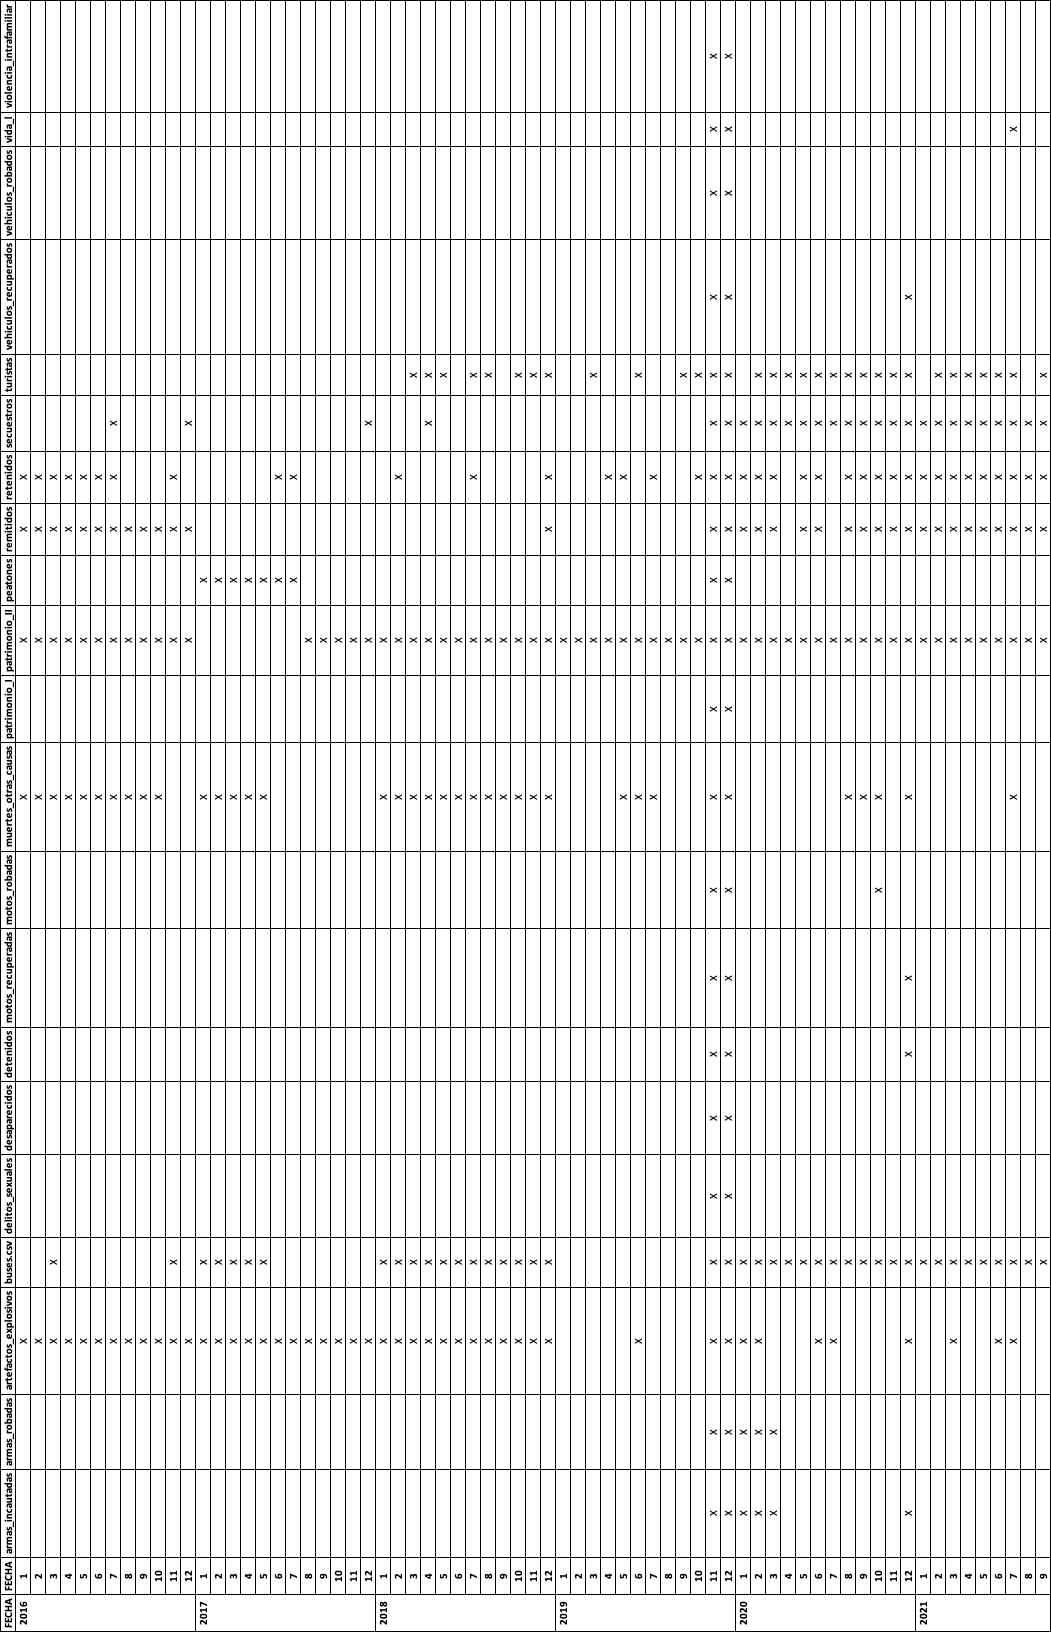
\includegraphics[scale=0.4]{Images/1}
	\caption{Adjunto en reporte.xlsx}
	\label{image:1}
\end{figure}

\begin{itemize}
	\item Los datos procesados y consolidados se encuentran en esta carpeta de Google Drive:\textbf{
	\href{https://drive.google.com/drive/folders/1wrUz2HQ4ot9iP2RcIvtUg_z284M36j6b?usp=sharing}{archivos}}. Dichos datos son los siguientes: 
	% Please add the following required packages to your document preamble:
	% \usepackage{booktabs}
	\begin{table}[H]
		\centering
		\caption{Datos analizados}
		\label{tab:datos}
		\begin{tabular}{@{}llllll@{}}
			&                       &                         & Archivos             &                         &                         \\ \midrule
			\multicolumn{1}{l|}{1} & Armas incautadas      & \multicolumn{1}{l|}{8}  & Motos recuperadas    & \multicolumn{1}{l|}{16} & Secuestros              \\
			\multicolumn{1}{l|}{2} & Armas robadas         & \multicolumn{1}{l|}{9}  & Motos robadas        & \multicolumn{1}{l|}{17} & Turistas                \\
			\multicolumn{1}{l|}{3} & Artefactos explosivos & \multicolumn{1}{l|}{10} & Muertes otras causas & \multicolumn{1}{l|}{18} & Vehículos recuperados   \\
			\multicolumn{1}{l|}{4} & Buses                 & \multicolumn{1}{l|}{11} & Patrimonio I         & \multicolumn{1}{l|}{19} & Vehículos robados       \\
			\multicolumn{1}{l|}{5} & Delitos sexuales      & \multicolumn{1}{l|}{12} & Patrimonio II        & \multicolumn{1}{l|}{20} & Vida                    \\
			\multicolumn{1}{l|}{6} & Desaparecidos         & \multicolumn{1}{l|}{13} & Peatones             & \multicolumn{1}{l|}{21} & Violencia intrafamiliar \\
			\multicolumn{1}{l|}{7} & Detenidos             & \multicolumn{1}{l|}{14} & Remitidos            & \multicolumn{1}{l|}{}   &                         \\
			\multicolumn{1}{l|}{8} & Motos recuperadas     & \multicolumn{1}{l|}{15} & Retenidos            & \multicolumn{1}{l|}{}   &                        
		\end{tabular}
	\end{table}
	\item Los datos, sin embargo, presentaban varios meses faltantes, los cuales se observan en \ref{image:1}. Donde las \textbf{X} representan los meses faltantes. Este cuadro se adjunta con los archivos anteriores en el archivo de \textbf{Reporte.xlsx}. 
	
	\subsection{Tratamiento}
	El tratamiento de los datos consistió en lo siguiente:
	\begin{itemize}
		\item Consolidación de las bases de datos del 2016 hasta la actualidad. 
		\item Eliminación de datos duplicados (preservando el más reciente). 
		\item Eliminación de columnas duplicadas. 
		\item Limpieza de datos general. 
	\end{itemize}
	
\end{itemize}




%---------------------------


\end{document}